%!TEX root = ../thesis.tex

% \vspace{-10pt}

\section{本章の概要}
本章では,\ref{sec:nav-sys}節でシステムの概要を示す.また,\ref{sec:real-robot}節で実ロボットにおける歩行者の位置計算の詳細,\ref{sec:nav-usage}節でナビゲーションにおける予測結果の利用方法について述べる.

\section{実験概要}
提案手法の有効性を評価するために,実際の環境でロボットと歩行者がどのように相互作用するかを観察し,提案手法を用いてその行動を予測する実験を行う.本実験には20代の男性4名が参加し,そのうちランダムに選ばれた2名のデータを予測用に使用する.

\section{実験方法}
本実験は,先行研究\cite{si2023-tanno}の実験を参考に行った.\figref{Fig:oculus-exp-overview}に示す屋内環境で実験を行った.\figref{fig:tracking-robot}に示す

\begin{figure}[H]
  \centering
 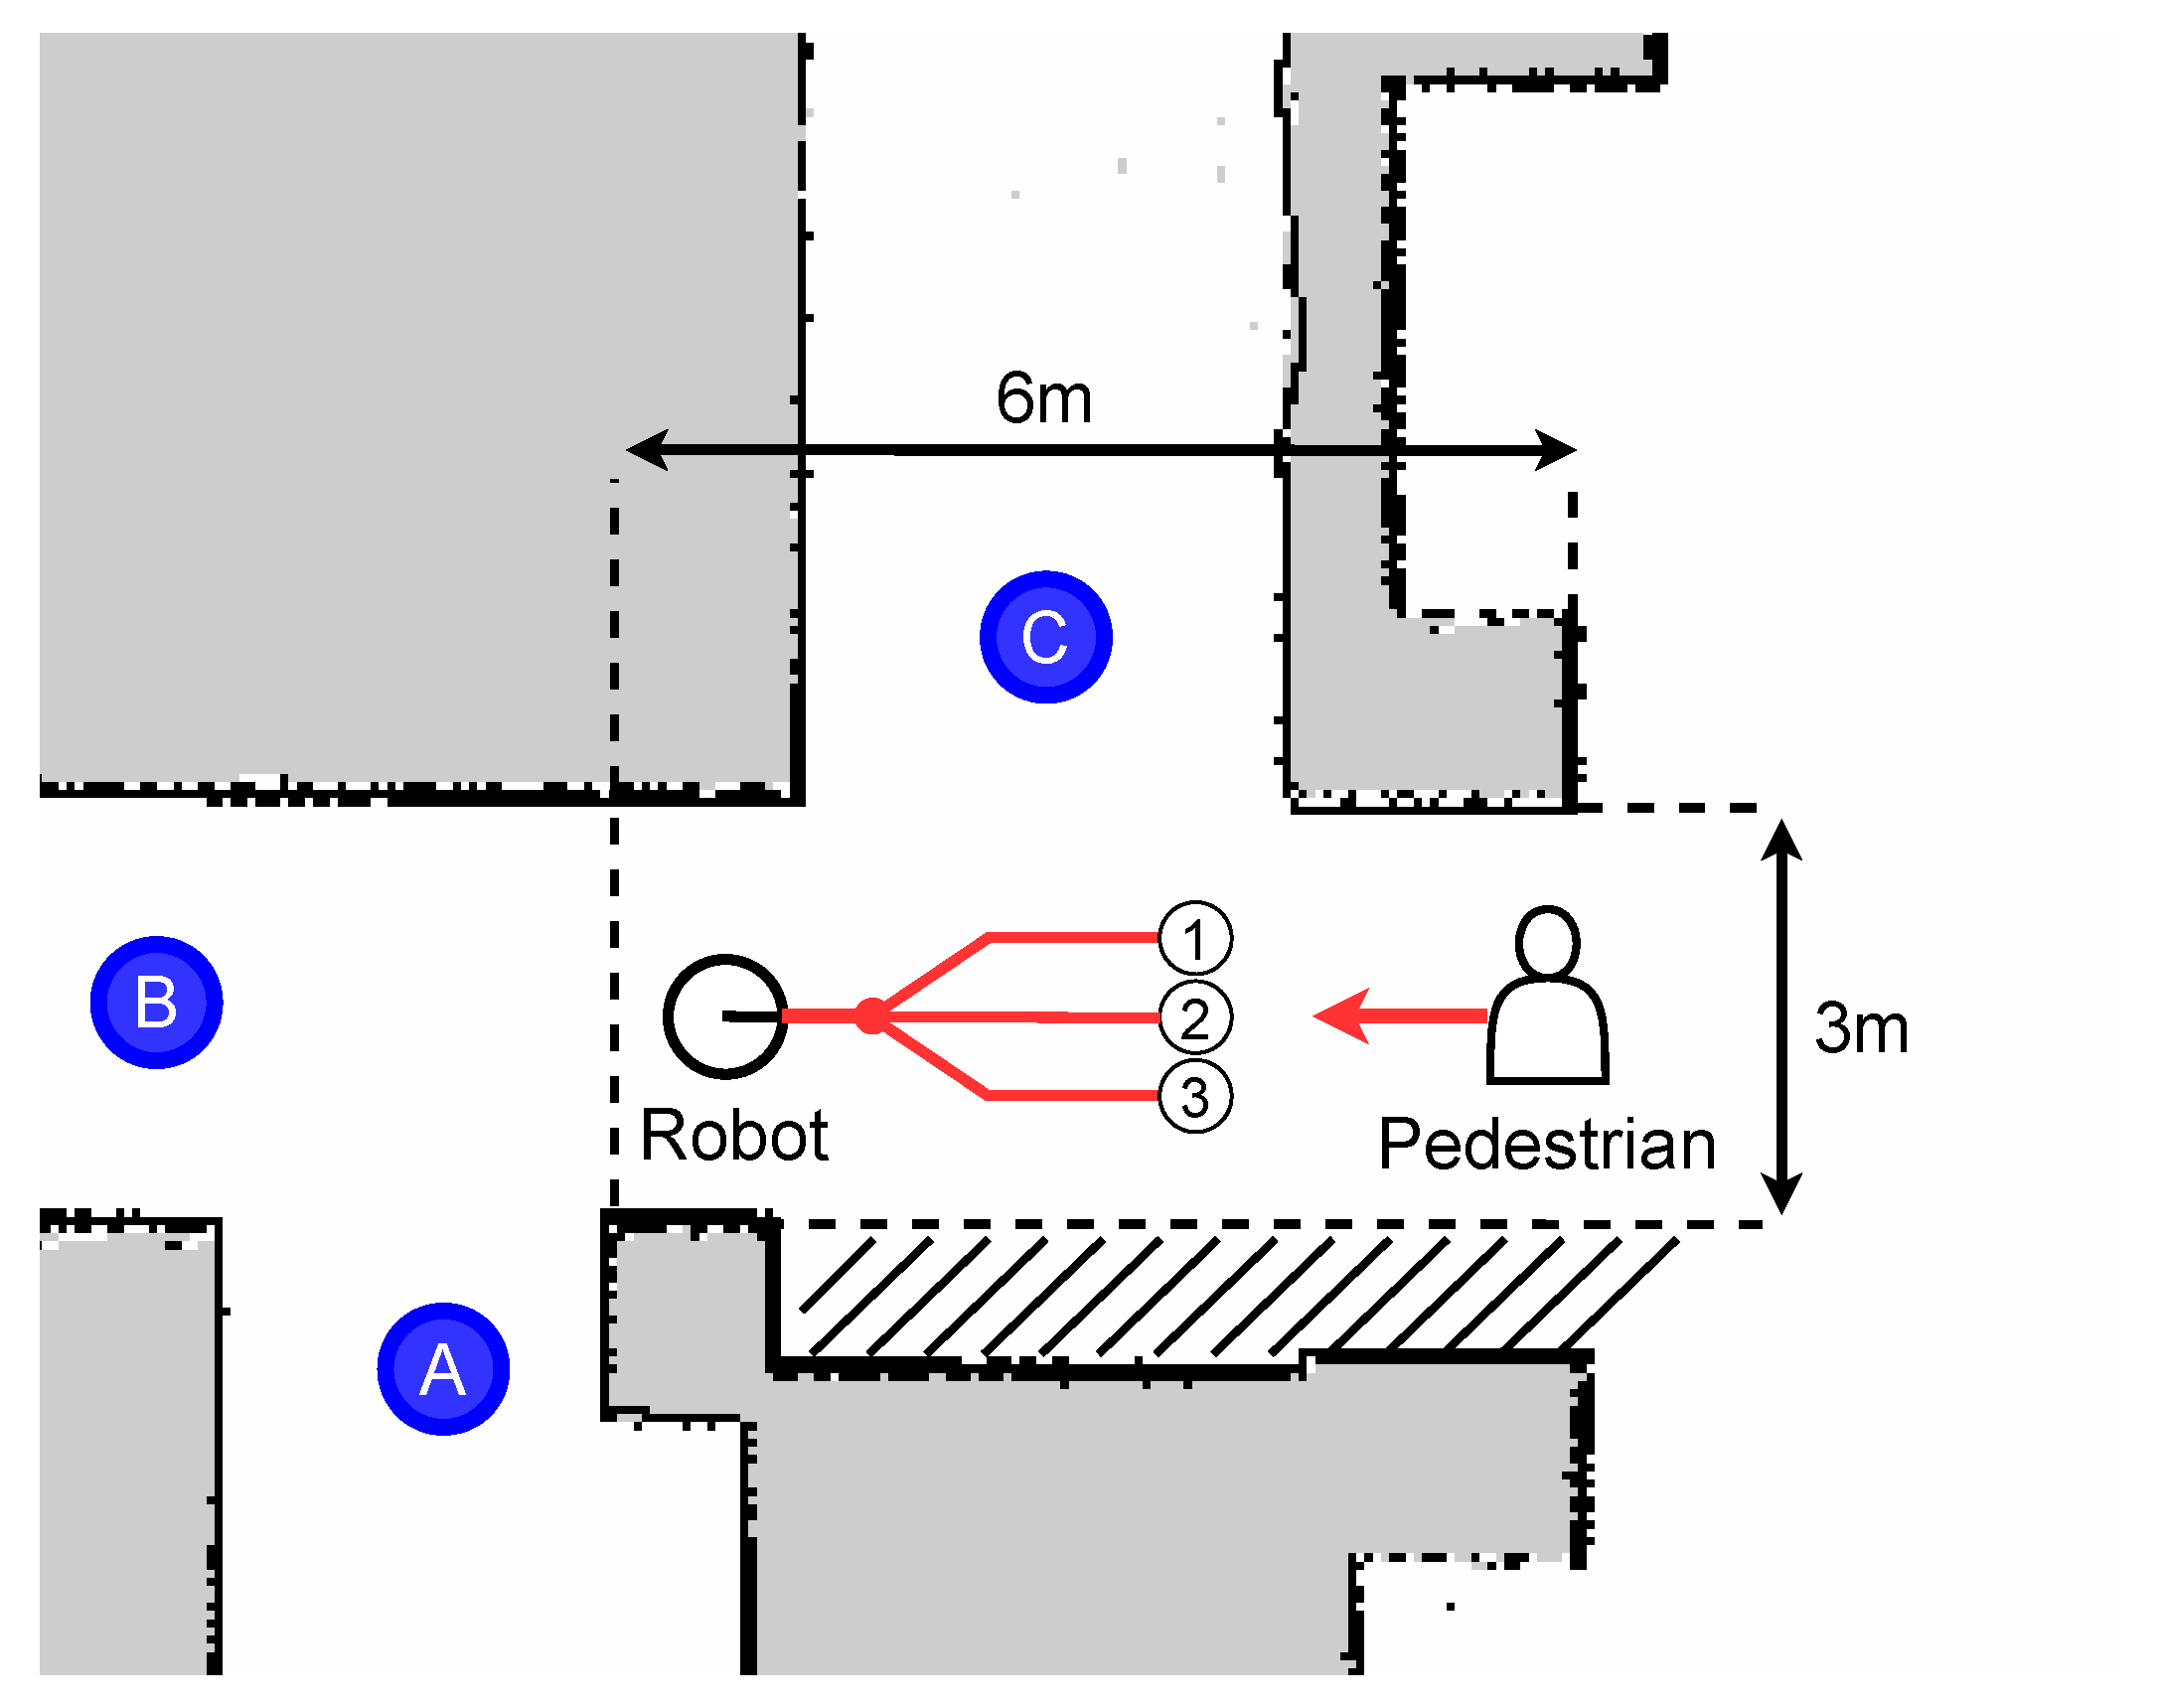
\includegraphics[keepaspectratio, scale=0.3]
      {images/oculus_experiments.pdf}
\caption{Experimental environment}
 \label{Fig:oculus-exp-overview}
\end{figure} 

\begin{figure}[H]
  \centering
  \begin{minipage}{0.45\textwidth}
    \centering
    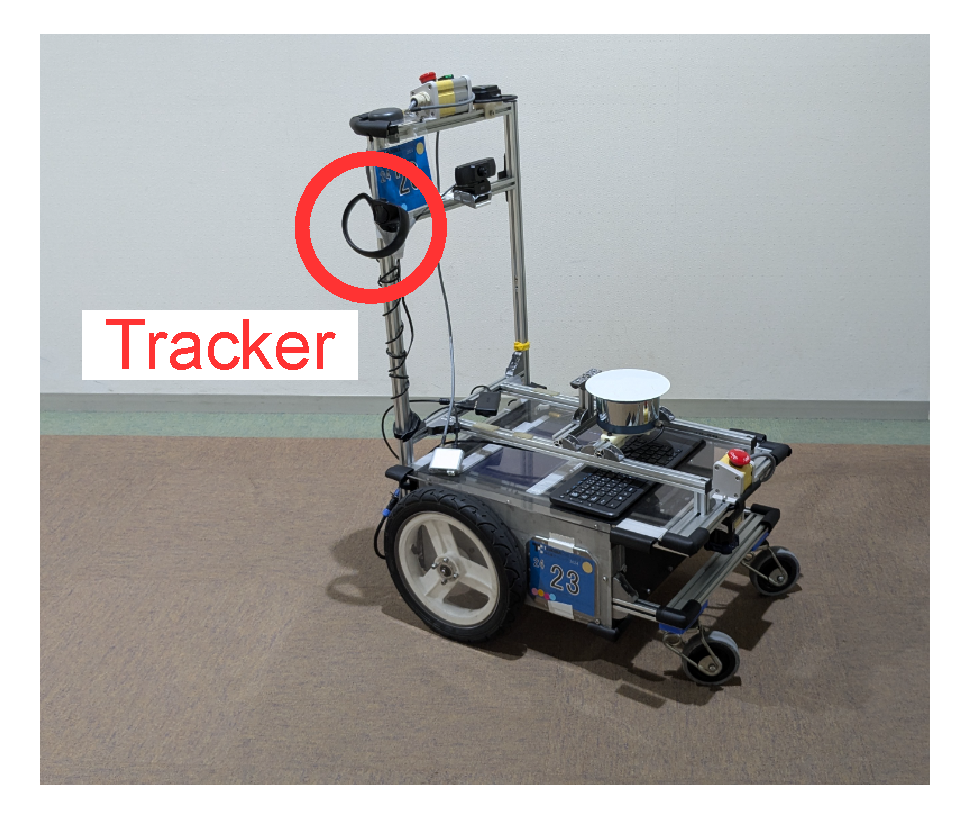
\includegraphics[width=\textwidth]{images/tracking-robot.pdf}
    \subcaption{Robot}
    \label{fig:tracking-robot}
  \end{minipage}
  % \hfill
  \begin{minipage}{0.45\textwidth}
    \centering
    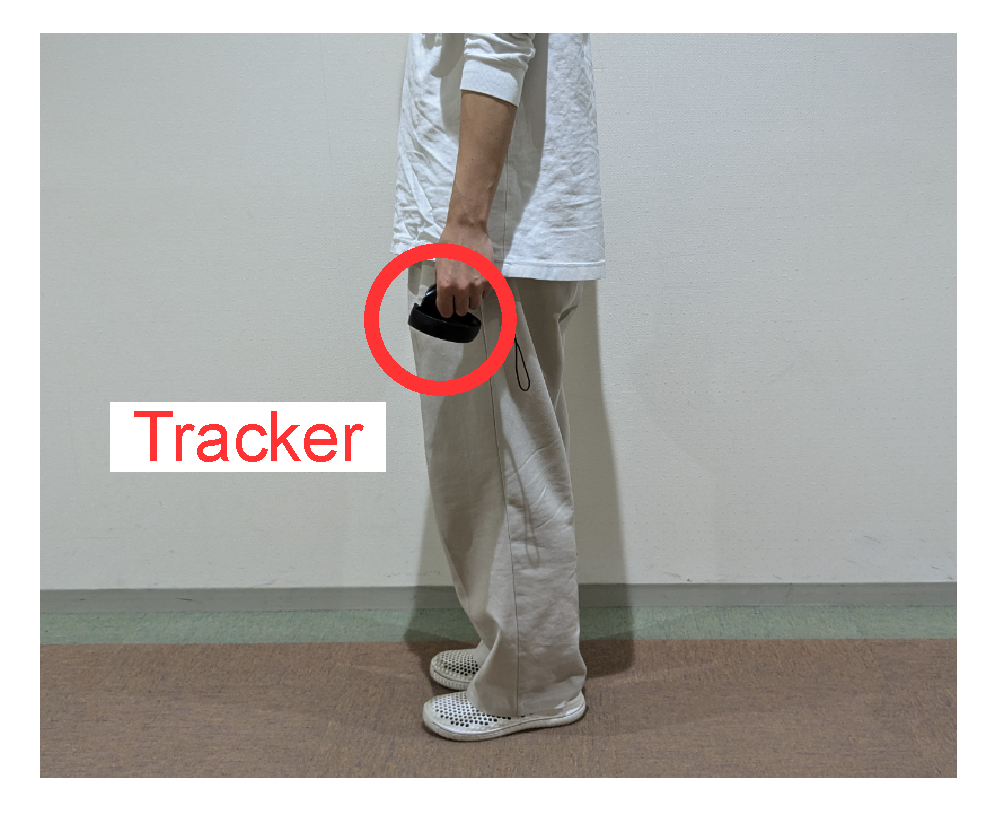
\includegraphics[width=\textwidth]{images/tracking-ped.pdf}
    \subcaption{Pedestrian}
    \label{fig:tracking-ped}
  \end{minipage}
  \caption{Tracking sensor setup}
  \label{fig:tracking}
\end{figure}

\section{結果と考察}

\newpage
